\Aufgabe[e]{Approximation der Flugbahn eines Projektils}{
Ein kugelförmiges Projektil mit einem Radius von 5 cm aus Stahl wird mit einer bestimmten Anfangsgeschwindigkeit 
$\vec v_0 = (v_{x,0}, v_{y,0})^T$ geworfen.
%
Die Flugbahn wird unter Berücksichtigung des Luftwiderstands approximiert.
Die Formel für die Luftwiderstandskraft lautet
$$
F = \frac12 c \rho A |\vec v|^2,
$$
wobei die Parameter in der Formel sind
\begin{itemize}
\item $c = 0.47 \quad [-]$: Luftwiderstandsbeiwert für ein kugelförmiges Projektil,
\item $A \quad [m^2]$: Querschnittsfläche des kugelförmigen Projektils,
\item $\rho=1.225 \quad [Kg/m^3]$: Dichte der Luft.
\end{itemize}

Die Flugbahn liegt in der xy-Ebene. Die Position des Projektils $\vec P(t)$ in der Zeit wird von beiden Komponenten des Positionsvektors bestimmt
$$
\vec P(t) = (x_p(t), y_p(t))^T.
$$
%
Wir sind nur an der x-Komponente interessiert, welche mit der folgenden Formel beschrieben werden kann
$$
x_p(t) = \frac{1}{\mu} \ln(1+\mu v_{x,0} t),
$$
wobei die Parameter in der Formel sind
\begin{itemize}
\item $\mu = \displaystyle \frac{1}{2m} c \rho A \quad [1/m]$,
\item $v_{x,0}= 60 \quad [m/s]$: x-Komponente der Anfangsgeschwindigkeit,
\item $m \quad [kg]$: Masse des Projektils, die unter Berücksichtigung der Dichte des Stahls, $\rho_s = 7.85 \, [gr/cm^3]$, bestimmt werden muss.
\end{itemize}

\begin{itemize}
\item Bestimmen Sie das Taylor-Polynom zweiter Ordnung $T_2(t)$, das die x-Komponente $x_p(t)$ der Flugbahn um den Zeitpunkt $t=0$ approximiert.
\item Berechnen Sie die Differenz zwischen der Position $x_p(t)$ des Projektils und seiner Taylor-Approximation $T_2(t)$ zum Zeitpunkt $t=10$: $d(t) = |T_2(t) - x_p(t)|$.
\item Bestimmen Sie das Restglied und geben Sie eine obere Schranke für seinen Betrag im Zeitintervall $t=[0,10]$ an. Vergleichen Sie dies mit der oben berechneten Differenz $d(10)$.
\end{itemize}
Hinweis: Man achtet auf die Einheiten!
}

\Loesung{
\begin{itemize}
\item Durchmesser der kreisformigen Querschnittsfläche: $D=10 \, cm = 0.1\, m$,
\item Querschnittsfläche $A = \pi D^2 / 4 \approx 0.0079\, m^2$,
\item Volumen der Kugel: $V = \pi D^3/6 \approx 5.236 \cdot 10^{-4}$,
\item Dichte des Stahls $\rho_s = 7.85 \, gr/cm^3 = 7850 kg/m^3$,
\item Masse der Kugel: $m = \rho_s V \approx 4.1103$,
\item $\mu \approx 5.5 \cdot 10^{-4}$.
\end{itemize}
Das Taylor-Polynom um den Zeitpunkt $t=0$ ist
$$
T_2(t) = x_p(0) + x_p'(0)\, x + \frac12 x_p''(0)\, x^2
$$
und das Restglied ist
$$
R_2(t,\xi) = \frac16 x_p'''(\xi)\, x^3.
$$
Die Ableitungen der Funktion $x_p$ sind
\begin{align*}
x_p'(t) &= \frac{v_{x,0}}{\mu\, v_{x,0}\, t+1},\\
x_p''(t) &= \frac{-\mu\, v^2_{x,0}}{\left(\mu\, v_{x,0}\, t+1\right)^2},\\
x_p'''(t) &= \frac{2\, \mu^2\, v^3_{x,0}}{\left(\mu\, v_{x,0}\, t+1\right)^3},
\end{align*}
und zum Zeitpunkt $t=0$ sind
\begin{align*}
x_p'(0) &= 60,\\
x_p''(0) &\approx -1.9803,\\
x_p'''(0) &\approx 0.1307.
\end{align*}
\begin{itemize}
\item Das Taylor-Polynom ist
$$
T_2(t) = 60\, x -1.9803\, x^2.
$$
\item Die Differenz in $t=10$ ist
$$
d(10) = | T_2(10) - x_p(10) | \approx 17.5117.
$$
\item Das Restglied ist
$$
R_2(t;\xi) = \frac{1}{6} \frac{0.1307}{(0.0330\, \xi +1)^3} \, x^3.
$$
Eine Abschätzung der Schranke bekommt man für $t=10$ und $\xi = 0$
$$
R_2(t;\xi) \leq \frac{1}{6} x_p'''(0)\, 10^3 \approx 21.7863
$$

\end{itemize}

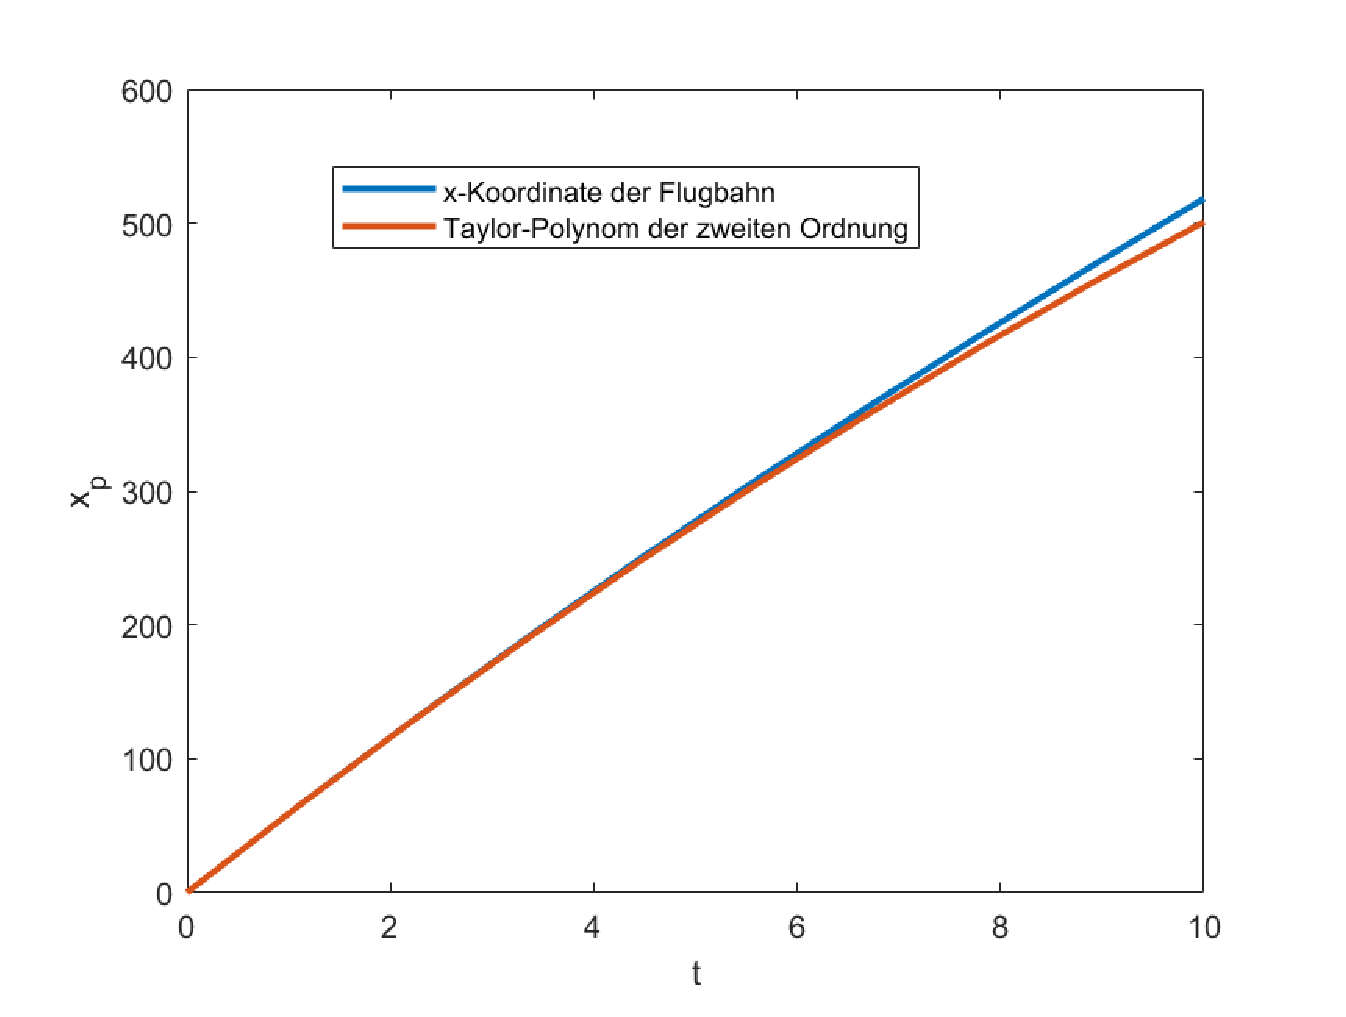
\includegraphics[width =0.5\textwidth]{../A/Wiederholung/plot_Flugbahn.eps}
}

\ErgebnisC{AufgFlugbahn}
{
Die Ableitungen der Funktion $x_p$ zum Zeitpunkt $t=0$ sind
\begin{align*}
x_p'(0) &= 60,\\
x_p''(0) &\approx -1.9803,\\
x_p'''(0) &\approx 0.1307.
\end{align*}

Die Differenz zwischen der Funktion $x_p$ und dem Taylor-Polynom zum Zeitpunkt $t=10$ ist
$$
d(10) = | T_2(10) - x_p(10) | \approx 17.5117.
$$

Graph der x-Koordinate der Flugbahn und des Taylor-Polynoms

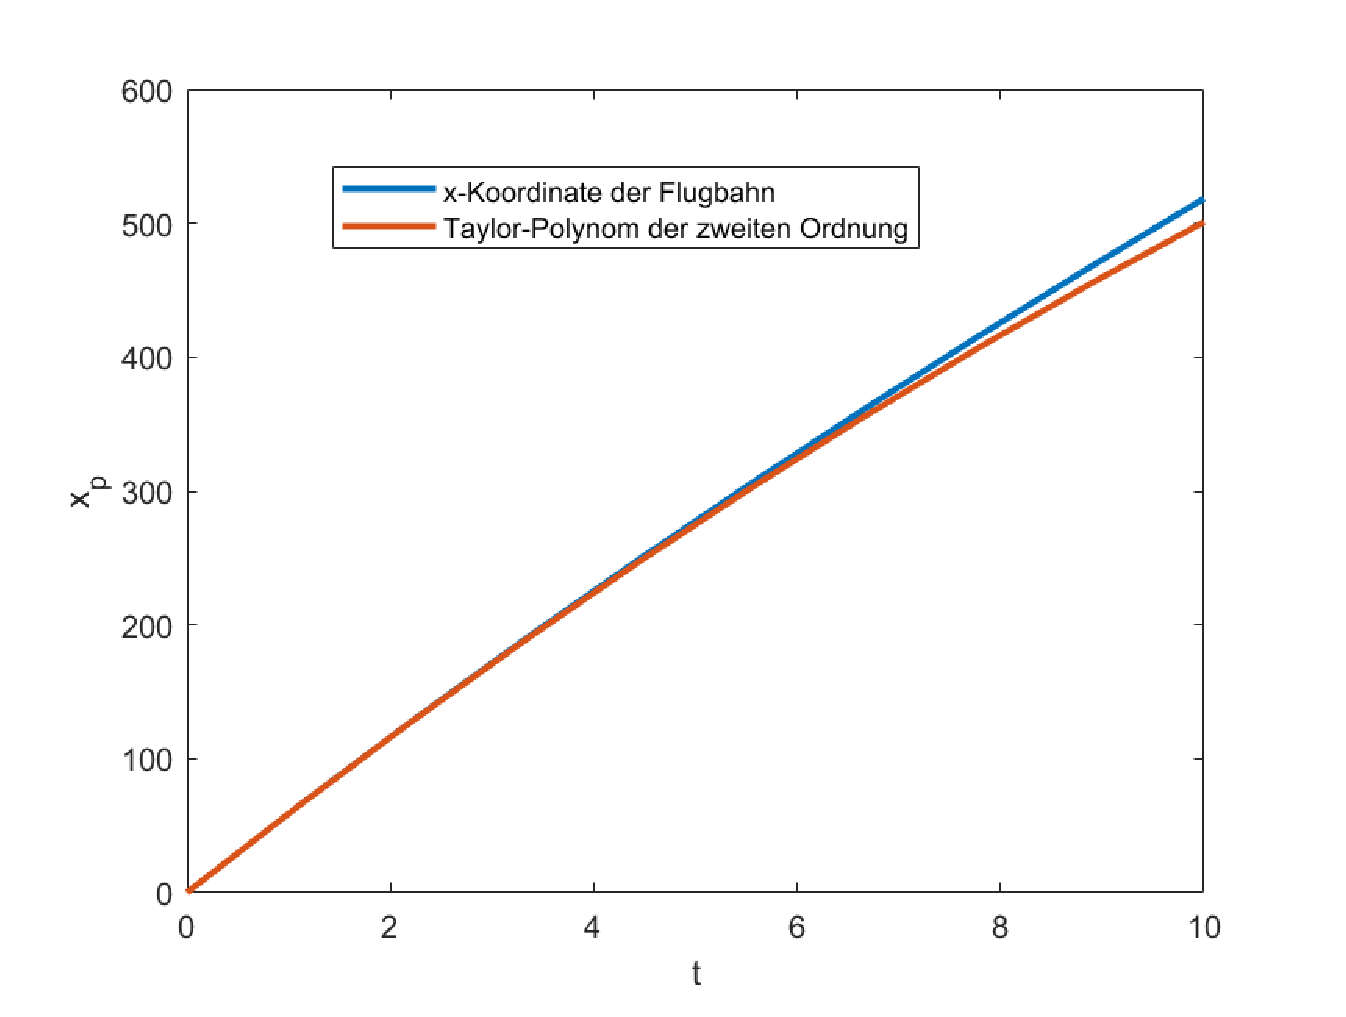
\includegraphics[width =0.5\textwidth]{../A/Wiederholung/plot_Flugbahn.eps}
}

